%%%%%%%%%%%%%%%%%%%%%%%%%%%%%%%%%%%%%%%%%%%%%%%%%%%%%%%%%%%%%%%%%%%%%%%%%%%%%%%%
% Chapter 4: Desarrollo
%%%%%%%%%%%%%%%%%%%%%%%%%%%%%%%%%%%%%%%%%%%%%%%%%%%%%%%%%%%%%%%%%%%%%%%%%%%%%%%%

%+++++++++++++++++++++++++++++++++++++++++++++++++++++++++++++++++++++++++++++++
% \section{Desarrollo con PlayStation Camera}
% \label{4:sec:2}

Una vez preparado el entorno de desarrollo: haber instalado y configurado ROS,
y posteriormente haber añadido PlayStation Camera solo falta recoger secuencias
de imágenes con la cámara. En esta sección se va a explicar como recoger
imágenes de la PlayStation Camera, para el análisis posterior de las mismas y
la reconstrucción del mapa 3D.

%+++++++++++++++++++++++++++++++++++++++++++++++++++++++++++++++++++++++++++++++
\subsection{Introducción}
Una primera aproximación del problema de la reconstrucción del mapa y la
localización en el mismo, es utilizar solamente PlayStation Camera. Haciendo
repaso de lo que se vio en el capítulo ~\ref{chapter:conceptos}, la odometría es
uno de los pilares de la navegación en robots. Sin embargo, la odometría es muy
susceptible a la acumulación de errores, por lo que es necesario contar con
todas las medidas necesarias para acotar estos problemas.

Utilizando solamente PlayStation Camera junto con un ordenador para recoger
muestras, la única odometría que tiene presencia es la odometría visual. Esto es
un punto muy a tener en cuenta en el desarrollo y las medidas que se planean
hacer.

Para simular el comportamiento de un robot, la cámara se integrará en un carro
industrial y estará conectado al ordenador encargado de recoger los datos
mediante ROS. Por otra parte, es necesario contar con un lugar de grabación
adecuado, en esta ocasión se hará uso de un hangar de tamaño medio en el que las
condiciones lumínicas son idóneas.

%+++++++++++++++++++++++++++++++++++++++++++++++++++++++++++++++++++++++++++++++
\subsection{Reconstrucción del mapa}
La idea general para la reconstrucción del mapa tridimensional es:

\begin{itemize}
  \item Recoger imágenes de las bolsas de datos
  \item Rectificación de las imágenes
  \item Cálculo de la disparidad y odometría
  \item Construir mapa a partir de la odometría
\end{itemize}

\begin{minipage}{\linewidth}
    \centering
    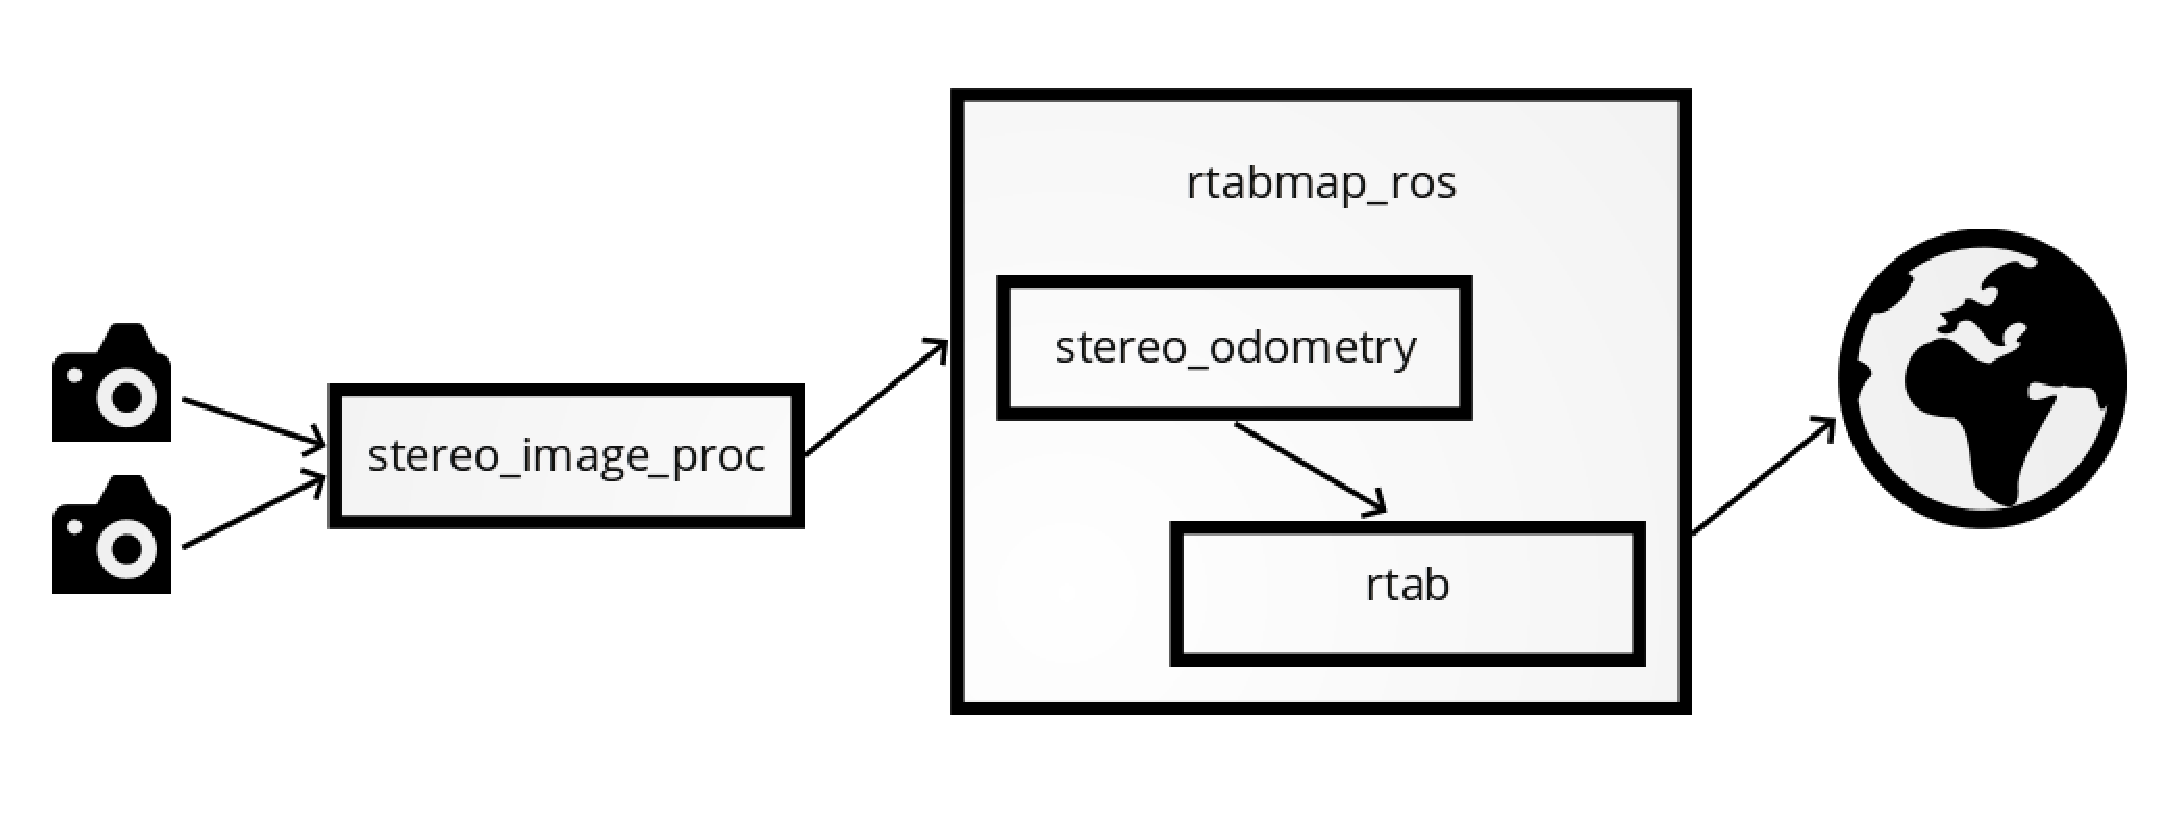
\includegraphics[width=0.8\textwidth]{images/cap4/Carro-esquema.eps}
    \captionof{figure}{Esquema de ROS para construir un mapa 3D}
    \label{fig:Carro-esquema}
\end{minipage}

%--------------------------------------
\paragraph{Rectificación} \hspace{0pt}

A partir del cálculo del mapa de disparidad a partir de las imágenes
rectificadas, es posible obtener una odometría visual. Volviendo a recordar uno
de los objetivos de ROS, este es un ejemplo de aquellas tareas que dificultan el
desarrollo de un robot. Para solucionar este problema ROS cuenta con un paquete
llamado \textit{``stereo\_image\_proc"} \cite{PackageStereoImageProc}.

Este paquete cuenta con un nodo que recibe el mismo nombre, el cuál tiene como
objetivo procesar las imágenes estéreo que recibe. El nodo está suscrito a
cuatro tópicos: \textit{``left/image\_raw"}, \textit{``'left/camera\_info"},
\textit{``right/image\_raw"} y \textit{``right/camera\_info"}, los cuales
corresponden con las imágenes en formato RAW sin comprimir de la cámara y los
metadatos asociadas a ellas.

Con el nodo ROS Master ejecutándose en segundo plano, para ejecutar el nodo
\textit{``stereo\_image\_proc"} basta con introducir en una terminal:
\\
\begin{lstlisting}
  $ rosrun stereo_image_proc stereo_image_proc __ns:=stereo
\end{lstlisting}

Mientras, el nodo se encarga de publicar varios tópicos como la imágenes en
grises, a color y las imágenes correctamente rectificadas, también está
preparado para publicar el mapa de disparidad y una nube de puntos. Tanto las
tareas de procesamiento de la rectificación, como la disparidad y la nube de
puntos son bajo demanda, por lo que si ningún nodo está suscrito a estos tópicos
no se utilizarán recursos para ejecutar las tareas.

Para poder visualizar las imágenes ya procesadas, es posible utilizar una de las
utilidades ya comentadas de RQt: \textit{``rqt\_image\_view"}
\cite{PackageRqtImageView}. En una terminal se introduce lo siguiente:
\\
\begin{lstlisting}
  $ rosrun image_view disparity_view image:=/stereo/disparity
\end{lstlisting}

El nodo \textit{``disparity\_view"} está preparado para mostrar los tópicos
correspondiente a los mensajes de tipo \textit{``stereo\_msgs/DisparityImage"}
publicados por \textit{``stereo\_image\_proc"} en el tópico
\textit{``/stereo/disparity"}. De esta forma como argumento se selecciona dicho
tópico. El resultado es una imagen de disparidad de color, en función del nivel
de disparidad presente en un punto concreto de las imágenes, el tono de color
sera diferente.

%--------------------------------------
\paragraph{Odometría} \hspace{0pt}

Teniendo ya las imágenes izquierda y derecha rectificadas, con el paquete
\textit{``rtabmap\_ros"} \cite{PackageRtabmapRos}es posible obtener la odometría
visual de las imágenes. Este paquete está basado en RTAB-Map, herramienta basada
en técnicas de SLAM para la detección de cierres de bucle en tiempo real. Cuenta
con muchas características, por lo que lo mejor es explicar alguno de los
principales de los nodos que dispone:

\begin{itemize}
  \item \textbf{rtabmap:} es el nodo principal del paquete, encargado de
  almacenar el grafo del mapa de forma incremental y optimizarlo cuando se
  detecta un cierre de bucle.
  \item \textbf{rtabmapviz:} interfaz gráfica para poder visualizar los
  resultados de rtabmap.
  \item \textbf{Visual Odometry:} nodo general para la obtención de la odometría
  visual, el cual se puede dividir en dos.
  \begin{enumerate}
    \item \textbf{rgbd\_odometry:} odometría basada en imágenes RGBD.
    \item \textbf{stereo\_odometry:} odometría basada en imágenes en estéreo.
  \end{enumerate}
\end{itemize}

Para obtener la odometría, y viendo que las imágenes que tenemos son
estereoscópicas, es necesario utilizar el nodo \textit{``stereo\_odometry"}.
Este nodo está suscrito a los tópicos de las imágenes rectificadas y a sus
metadatos, y el resultado es un tópico de tipo \textit{``nav\_msgs/Odometry"}.

Con la odometría lista, faltaría la reconstrucción del mapa en 3D. El nodo
principal es el encargado de esta tarea, a partir de la odometría y la
transformación de coordenadas correspondiente, teniendo como resultado el tópico
\textit{``rtabmap\_ros/MapData"} con toda la información acerca del mapa.

Para lanzar el paquete \textit{``rtabmap\_ros"} es necesario introducir en una
terminal:
\\
\begin{lstlisting}
  $ roslaunch myps4eye carrito.launch
\end{lstlisting}

La utilidad \textit{``roslaunch"} permite cargar un archivo de este tipo. Se
trata de un archivo basado en XML en el que se definen los paquetes, los nodos y
las opciones que se desean lanzar, en vez de ser ejecutadas directamente desde
terminal. Se trata de la mejor opción cuando se desean lanzar muchos nodos a los
cuáles hay además que modificar sus parámetros.

Este launch puede encontrarse en el anexo ~\ref{appendix:carrito}, y en él se
puede ver como se lanzan los nodos \textit{``stereo\_odometry"} y
\textit{``rtabmap"} de \textit{``'rtabmap\_ros"}, y de forma opcional también el
nodo \textit{``rtabmapviz"} y otros paquetes de visualización como
\textit{``rviz"} y el paquete \textit{``tf"}.

El paquete \textit{``tf"} \cite{PackageTf}se encarga de determinar las
coordenadas de transformación de cada uno de los elementos de un robot. El nodo
\textit{``static\_transform\_publisher"} se encarga de realizar una
transformación de coordenadas a partir de los ejes x,y,z.

%--------------------------------------
\paragraph{Reconstrucción y visualización} \hspace{0pt}

Con \textit{``rtabmap"} o \textit{``rtabmapviz"} se puede seleccionar dos modos
de trabajo: construcción o localización. Para poder localizarse, es necesario
tener un mapa construido previamente. Lanzando el launch anterior se puede
observar en \textit{``rtabmapviz"} como se va generando el mapa que las imágenes
de PlayStation Camera van registrando en base a la odometría. La reconstrucción
del mapa se puede realizar en tiempo real o con bolsas de datos con secuencias
ya grabadas. En tal caso, solo bastaría con reproducir la bolsa para poder
generar el mapa:
\\
\begin{lstlisting}
  $ rosbag play --clock carrito.bag
\end{lstlisting}

El mapa es generado mediante una nube de puntos. Además de la nube de puntos, se
puede observar también como \textit{``rtabmap"} tiene presente el cálculo de
cierres de bucle. De esta forma, si se utiliza una secuencia donde se produce se
comienza desde un punto determinado, y se acaba volviendo al mismo punto,
\textit{``rtabmap"} se encargará de detectar este cierre para poder optimizar el
mapa.

\begin{minipage}{\linewidth}
    \centering
    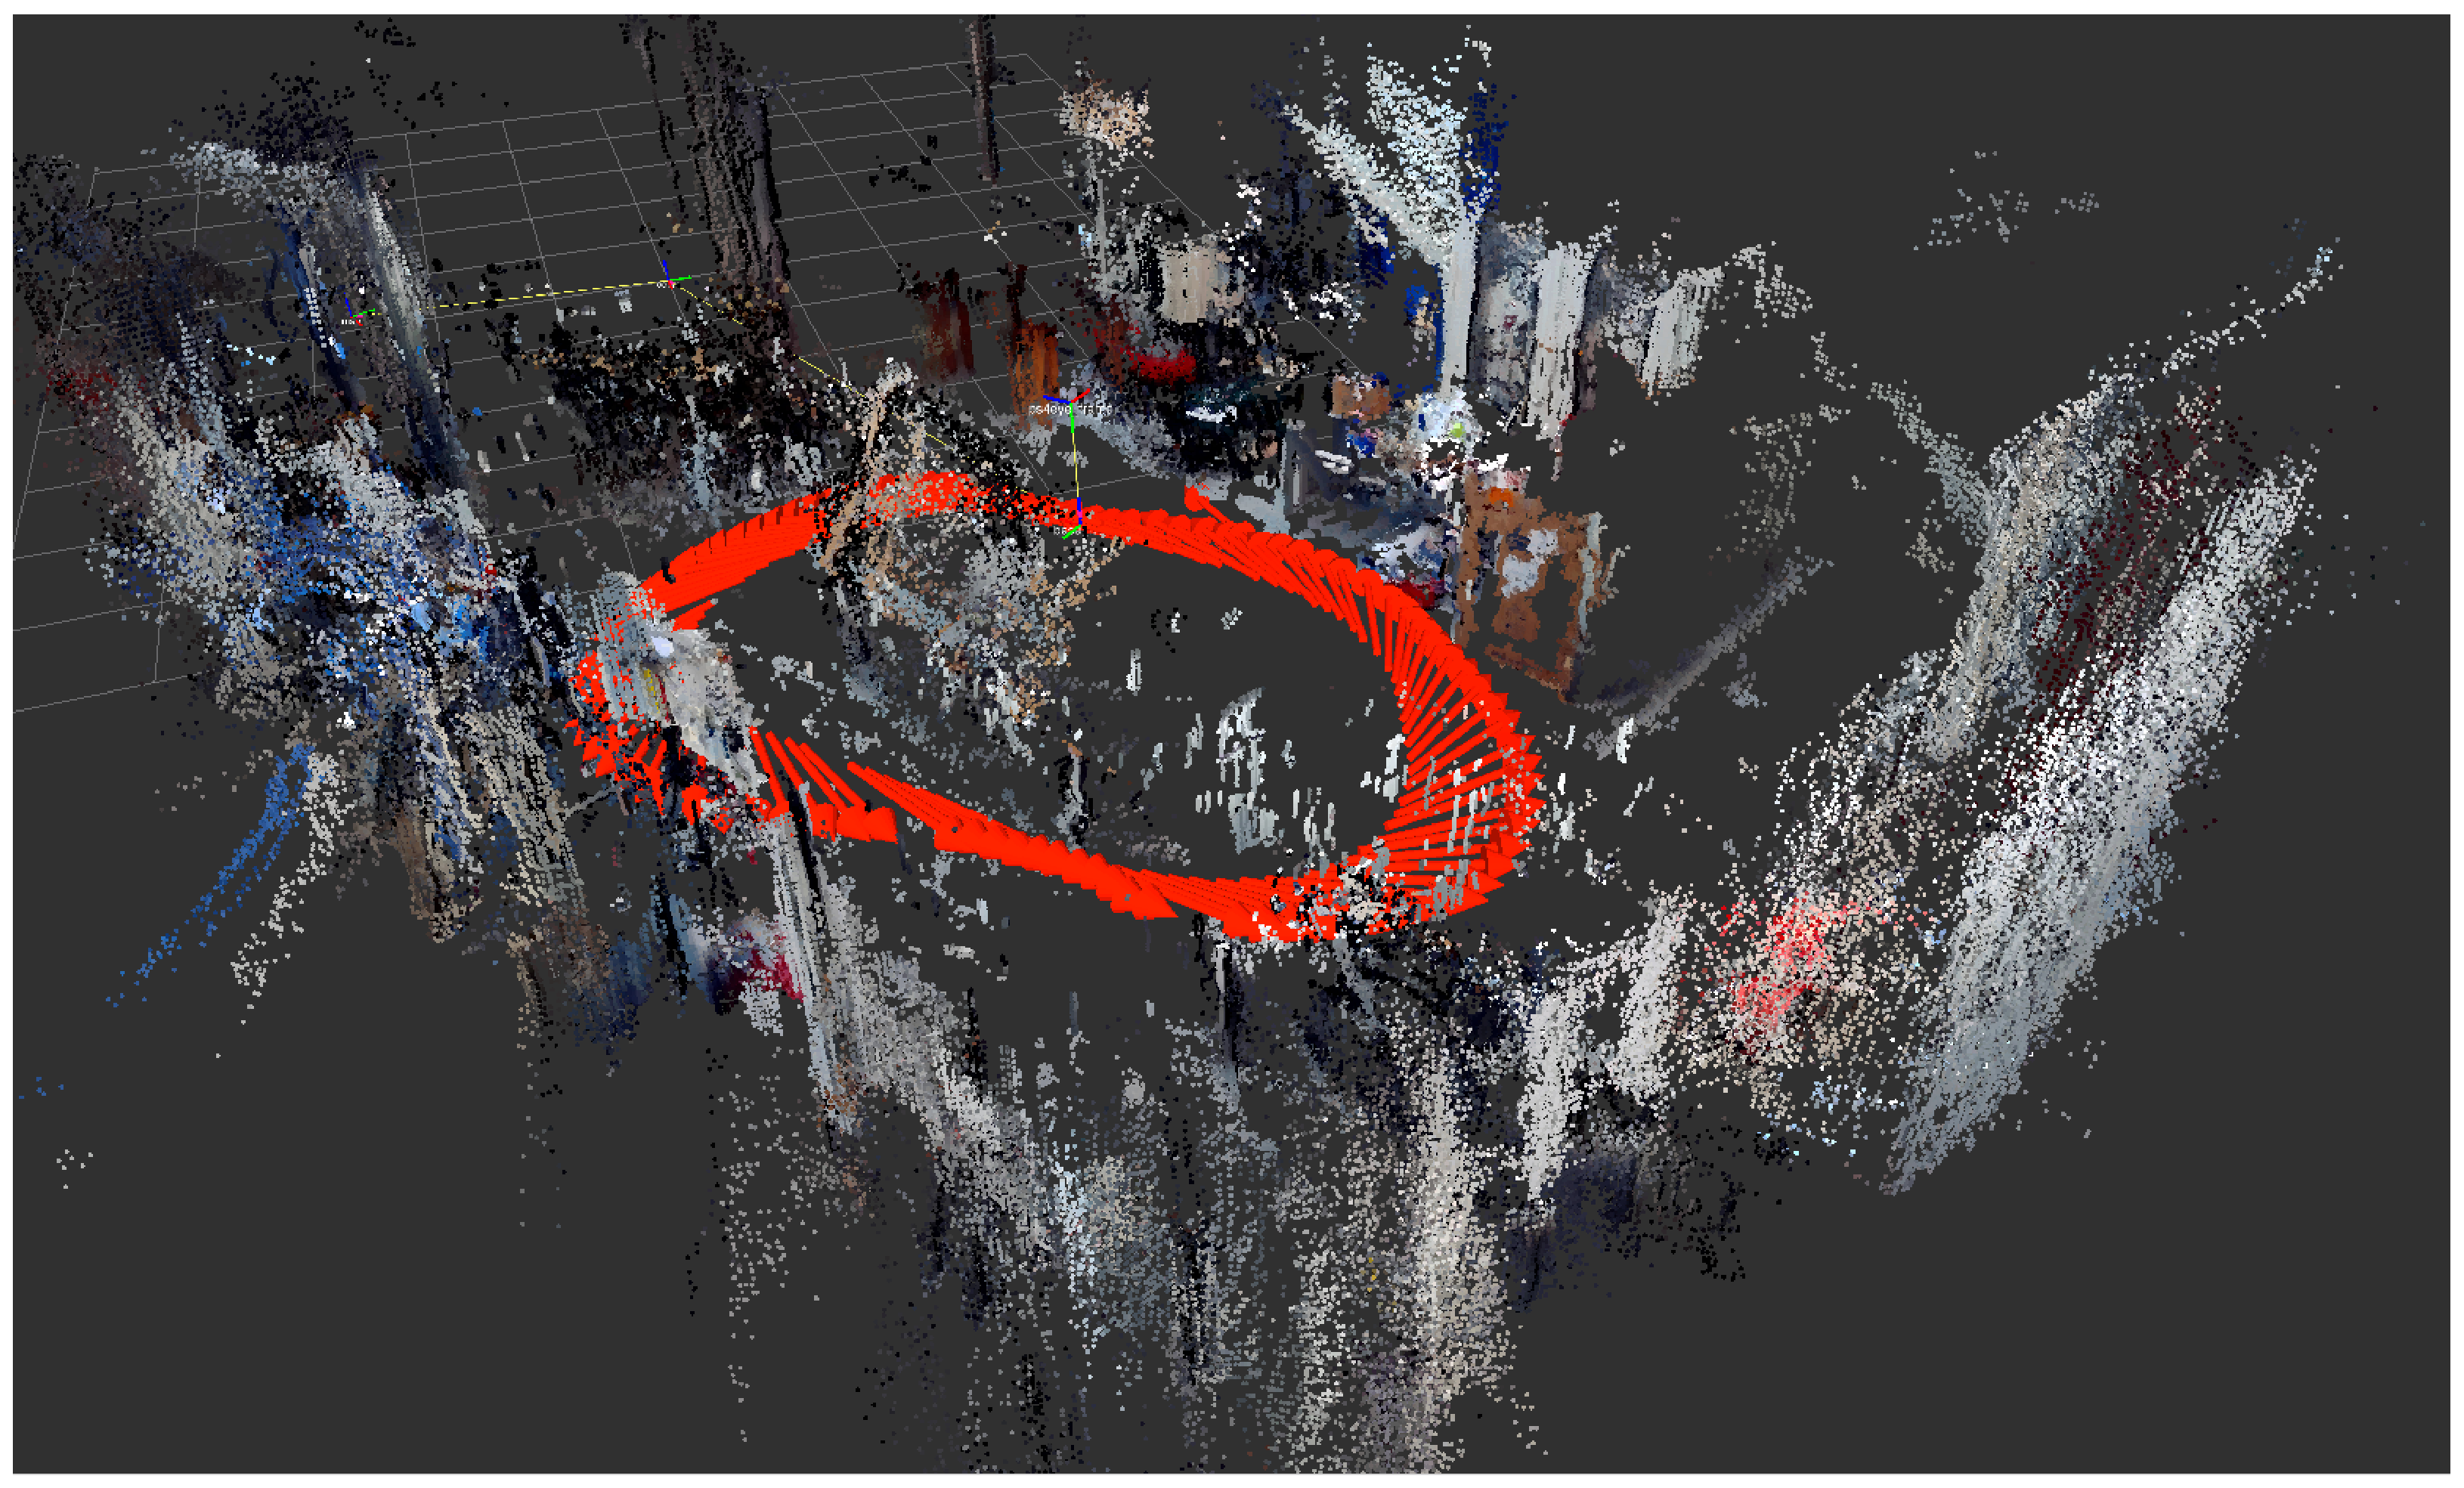
\includegraphics[width=0.8\textwidth]{images/cap4/rviz.eps}
    \captionof{figure}{Reconstrucción 3D del mapa en Rviz}
    \label{fig:Reconstruccion-Rviz}
\end{minipage}

Tras haber construido el mapa, los resultados pueden visualizarse con
\textit{``rviz"}. En la figura ~\ref{fig:Reconstruccion-Rviz} se puede observar
como se ve la nube de puntos que representa al mapa 3D y la odometría del Robot.
En este caso se dio dos vueltas alrededor de la misma estructura.

%+++++++++++++++++++++++++++++++++++++++++++++++++++++++++++++++++++++++++++++++
\subsection{Ajuste de parámetros}
El paquete \textit{``stereo\_image\_proc"} cuenta con una serie de parámetros
que pueden modificarse de manera dinámica utilizando la herramienta
\textit{``rqt\_reconfigure"}. Para lanzarlo se escribe en una terminal:
\\
\begin{lstlisting}
  $ rosrun rqt_reconfigure rqt_reconfigure
\end{lstlisting}

Gracias a esto podemos obtener mejores resultados. Aquí una pequeña descripción:

\begin{itemize}
  \item \textbf{Prefiltrado:}
  \begin{enumerate}
    \item \textbf{prefilter\_size:} tamaño de normalización de la imagen.
    \item \textbf{prefilter\_cap:} cota normalizada de los píxeles.
  \end{enumerate}
  \item \textbf{Correspondencia:}
  \begin{enumerate}
    \item \textbf{correlation\_window\_size:} diferencia de disparidad. 
    \item \textbf{min\_disparity:} valor mínimo de disparidad.
    \item \textbf{disparity\_range:} número de disparidades que buscar.
  \end{enumerate}
  \item \textbf{Postfiltrado:}
  \begin{enumerate}
    \item \textbf{uniqueness\_ratio:} filtro de sigularidades.
    \item \textbf{texture\_threshold:} disminución del ruido de fondo.
    \item \textbf{speckle\_size:} tamaño mínimo de las regiones a calcular.
    \item \textbf{speckle\_range:} máxima diferencia entre disparidades.
  \end{enumerate}
\end{itemize}

%+++++++++++++++++++++++++++++++++++++++++++++++++++++++++++++++++++++++++++++++
\subsection{Conclusiones}
Tras obtener el mapa y la odometría, el resultado no dista demasiado de la
realidad. Sin embargo hay que tener en cuenta de que se ha trabajado en un
entorno con las condiciones lumínicas necesarias y donde el espacio recorrido ha
sido muy pequeño.

La odometría visual es suficiente para conseguir resultados aceptables,
sobretodo en ambientes exteriores donde otros sistemas como los RGB-D (Kinect)
no pueden trabajar correctamente, pero si se sale de ambientes controlados con
picos de luz como en el exterior con mucho sol o en interiores con poca
luminosidad, los resultados pueden no tener el efecto esperado.

Es por ello, que habitualmente se utilizan más información para contrastar la
odometría visual, como los sistemas de odometría que utiliza la silla del
proyecto Perenquén.

%+++++++++++++++++++++++++++++++++++++++++++++++++++++++++++++++++++++++++++++++
